\chapter{Methods}\label{chap:methods}

\subsection{Data Collection}

We initiated the data collection process by scraping GitHub repositories. 
Utilizing web scraping techniques, we gathered data from 2000 repositories, encompassing a diverse range of projects. 
The default amount of repositories was 100000, which is a considerable amount. 
Considering our time constraints and the need for a more efficient process, we made the decision to change the default steps to 2000, keeping you informed and involved in the process. \ref{fig:srapingLabel}

As we worked on \textbf{scrapingGithub.py} file, we have faced the following issues. The solutions are also mentioned in below:
\begin{itemize}
    \item Missing \textbf{requests} library solved with \textit{ pip install requests }
    \item Missing \textbf{requests\_oauthlib} library, solved with  \textit{pip install requests\_oauthlib}
    \item Missing \textbf{all\_commits} file which we created manually.
    \item Missing Github Access Token, we generated through Github and save to \textbf{access} file inside the project folder. 
    \item Requests needed exception handling in case of losing the network.
\end{itemize}

After solving the above issue, they successfully ran the \textbf{scrapingGithub.py}, and its results were saved in \textbf{allcommits.json} file.

\begin{figure}
    \centering
    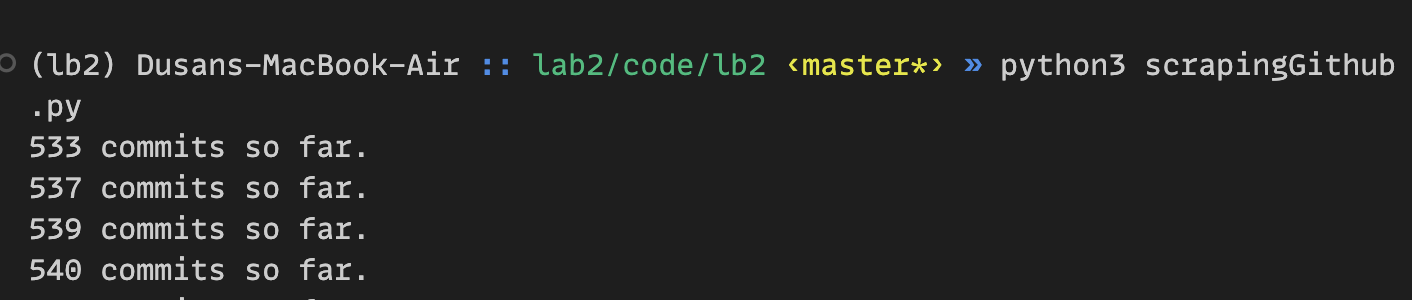
\includegraphics[width=0.5\linewidth]{Screenshot 2024-05-12 at 10.42.04.png}
    \caption{Gathering repositories}
    \label{fig:srapingLabel}
\end{figure}


\subsection{Keyword Filtering}

Following data collection, we performed keyword filtering to refine the dataset with \textbf{filterShowcase.py} file. 
By examining the names and readme files of the scraped repositories, we identified and filtered out repositories that matched our predefined keywords.
We have filtered the following showcases:
\begin{itemize}
    \item toomuchsecurity = ['offensive', 'pentest', 'vulnerab', 'security', 'hack', 'exploit', 'ctf ', ' ctf', 'capture the flag','attack'] 
    \item alittletoomuch = ['offensive security', 'pentest', 'exploits', 'vulnerability research', 'hacking', 'security framework', 'vulnerability database', 'simulated attack', 'security research'] 
    \end{itemize}

\subsection{Language Segregation}

With the help of \textbf{getDiffs.py} class file, we refined the dataset by segregating libraries with Python code from those without. 
This step was crucial for our subsequent analysis, focusing specifically on repositories containing Python code.
During this process, we faced the following issues:

\begin{itemize}
    \item missing os library which resolved by \textit{import os} \ref{fig:diff_os}.
    \item \textbf{datata} typo in line 110, which resolved by changing to \textbf{data} \ref{fig:diff_typo}.
\end{itemize}

\begin{figure}
    \centering
    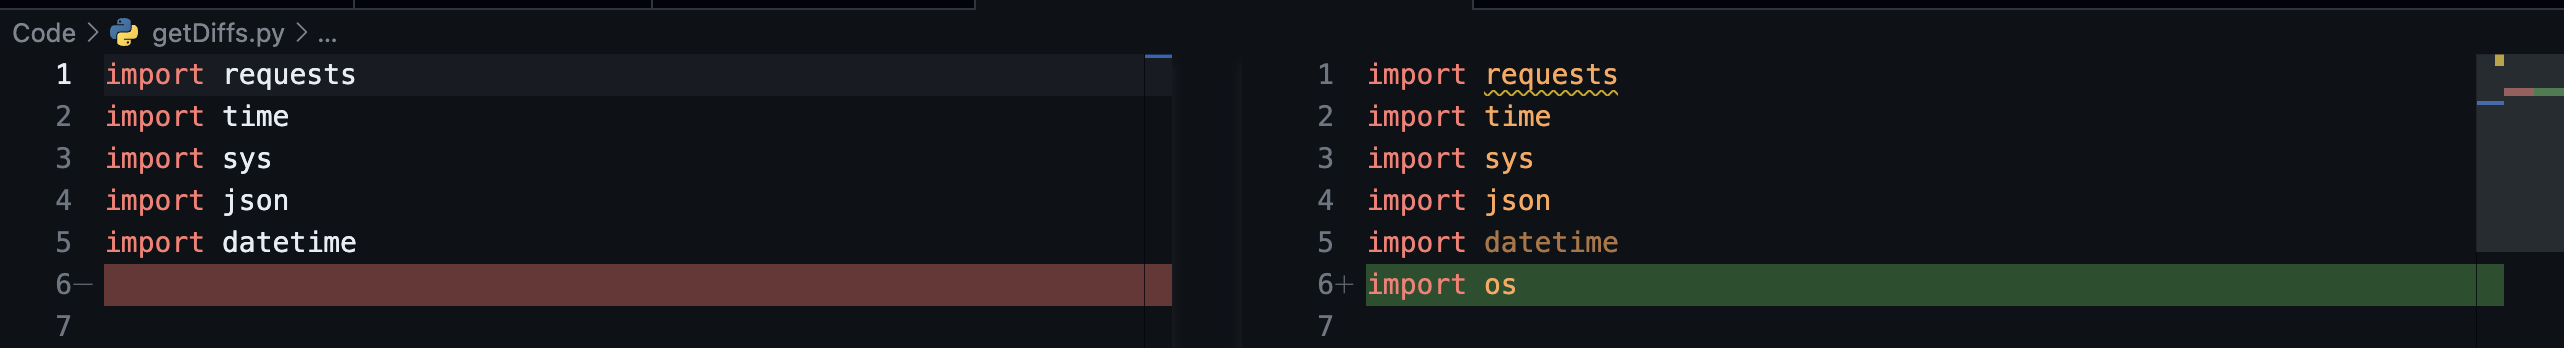
\includegraphics[width=1\linewidth]{getDiffe_os.png}
    \caption{GetDiffs missing os}
    \label{fig:diff_os}
\end{figure}

\begin{figure}
    \centering
    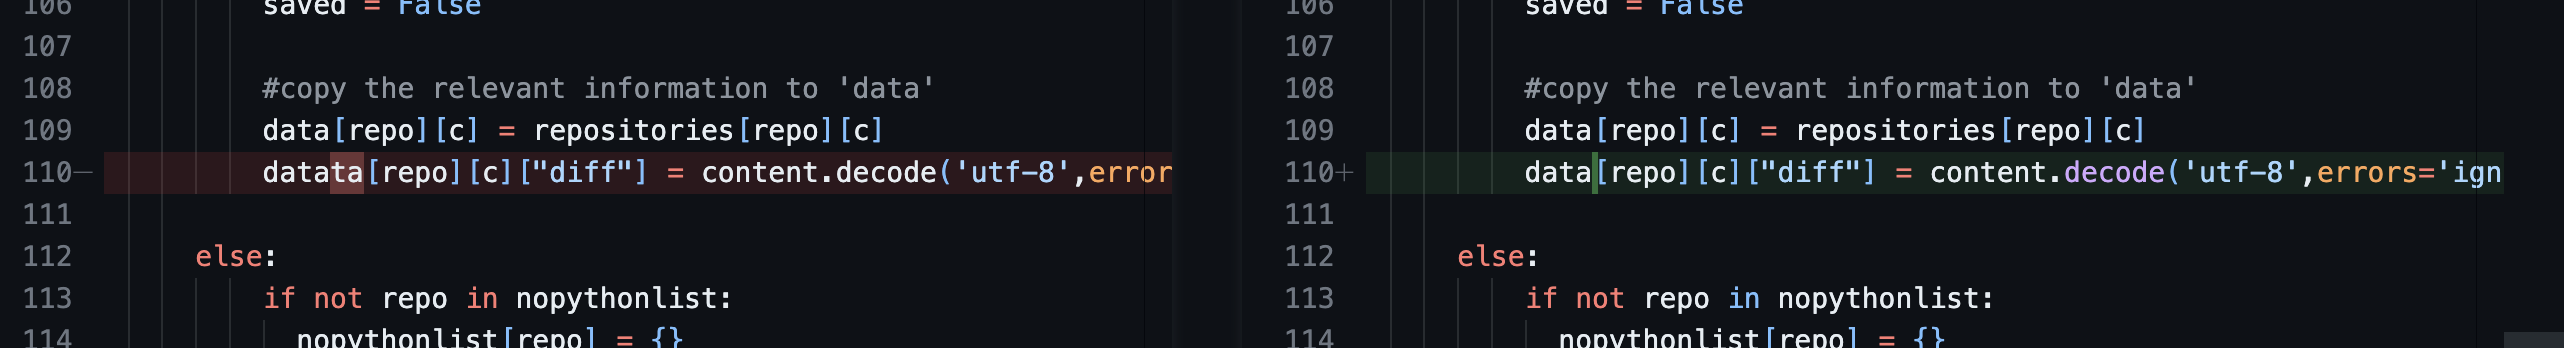
\includegraphics[width=1\linewidth]{getDiffs_typo.png}
    \caption{GetDiffs typo issue}
    \label{fig:diff_typo}
\end{figure}

\subsection{Commit Analysis}

In this step, we meticulously analyzed and downloaded the commits of the filtered repositories with the help of the \textbf{getData.py} file. 
By extracting all differences from their commits, we gained insights into the projects' evolution and the changes made over time.
We faced with only one issue in this phase \textit{ModuleNotFoundError: No module named 'keras.layers.convolutional'} which resolved by \textit{pip install keras} and the rest of code worked ideally and saved the result in \textbf{PyCommitsWithDiffs.json} JSON file.

\subsection{Dataset Acquisition}

To augment our dataset, we procured additional data from the main repository. 
This supplementary dataset, provided by the main repository, was essential for enhancing the depth and scope of our analysis in subsequent stages.

\subsection{Model Training}

The final step involved training our model based on the augmented dataset acquired in the previous step. This step handled with the help \textbf{makemodel.py}.
The Python script is a machine learning pipeline for training and evaluating an LSTM (Long Short-Term Memory) model for identifying vulnerabilities. 
We have trained the model over four types of vulnerabilities, XSS (Cross-Site Scripting), Path Disclosure, Remote Code Execution. The model specification 
is 10 for minimum count, 200 for iterations, 300 for vector size.

While working with this script we have faced the following issues due to library deprecations and changes in the Python version:

\begin{enumerate}

    \item \textbf{Sklearn.util class\_weight} issue which the input parameters changed in the latest verions. The differences shown in the figure \ref{fig:sklearn_class_wight}.
    \item \textbf{AttributeError: The vocab attribute was removed from KeyedVector in Gensim 4.0.0.}, the solution is changing vocab to \textbf{key\_to\_index}.
    \item \textbf{vector = w2v\_model[t] 'Word2Vec' object is not subscriptable} resolved by changing \textit{w2v\_model} to \textit{m2v\_model.wv}.
    \item \textbf{yhat\_classes = model.predict\_classes(X\_train, verbose=0)} issue because of the ... add in here . 
    Therefore we have changed to the \textbf{predict=model.predict(X\_train) yhat\_classes=numpy.argmax(predict,axis=1)}. 
    The final result for this changes shown in figure \ref{fig:yhat_changes}.
    % MARK: talk with atiq about it
    \item \textbf{numpy.core.\_exceptions.\_arraymemoryerror: unable to allocate 2.42 gib for an array with shape (8277, 131, 300) and data type float64} memory issue, we solved this issue with increasing virtual memory to 150 GB and GPU with the help of Tensorflow GPU library.

\end{enumerate}

Figures \ref{fig:makemodel1}, \ref{fig:makemodel2} and \ref{fig:makemodel3} log of each step for execution of this step. 

MARK TODO: Talk Abount the code enhancemnt you have and check if I miss something with ATIQullah

\begin{figure}
    \centering
    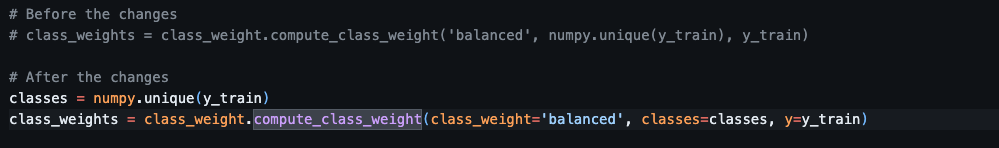
\includegraphics[width=1\linewidth]{sk-classweight.png}
    \caption{Sklearn Utils Class Weight}
    \label{fig:sklearn_class_wight}
\end{figure}

\begin{figure}
    \centering
    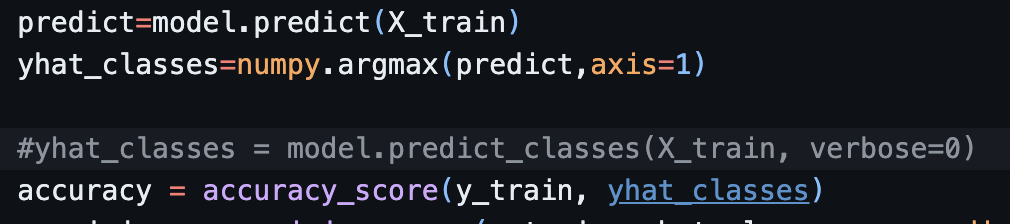
\includegraphics[width=1\linewidth]{yhat_changes.png}
    \caption{Yhat Changes}
    \label{fig:yhat_changes}
\end{figure}

\begin{figure}
    \centering
    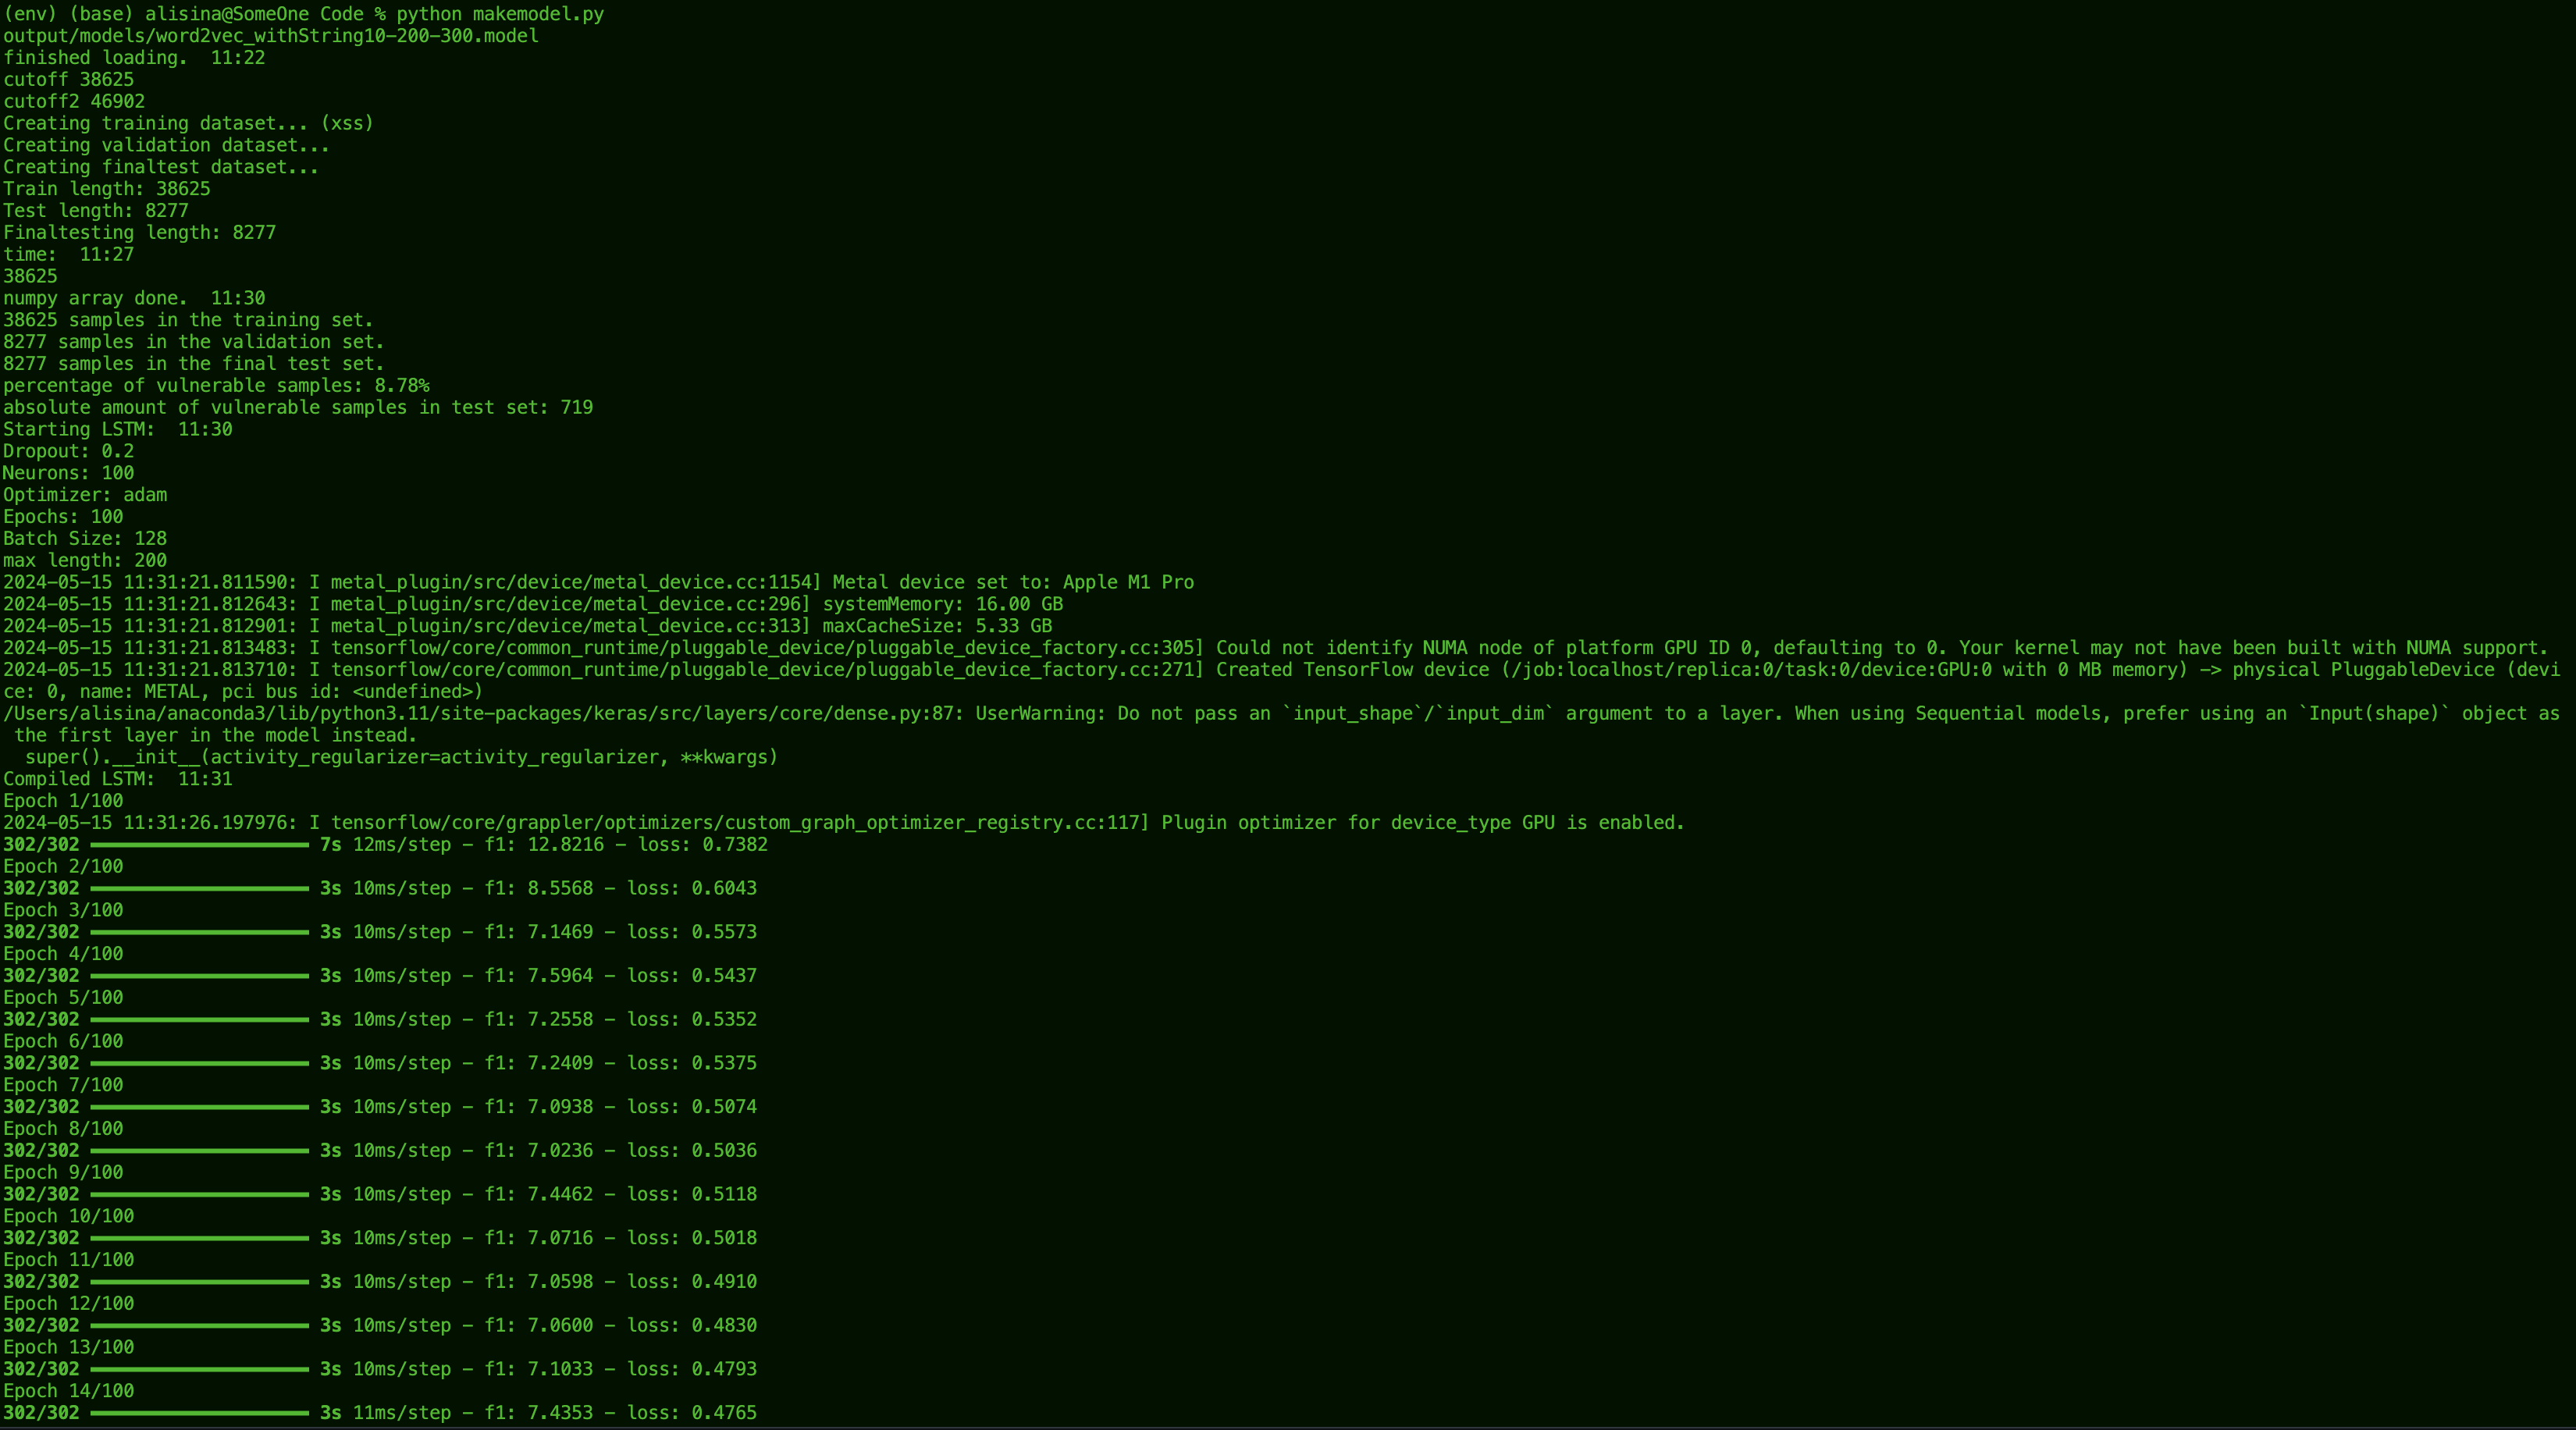
\includegraphics[width=1\linewidth]{makemodel1.png}
    \caption{Loading Data, Filtering Array \& Perpairing Data}
    \label{fig:makemodel1}
\end{figure}

\begin{figure}
    \centering
    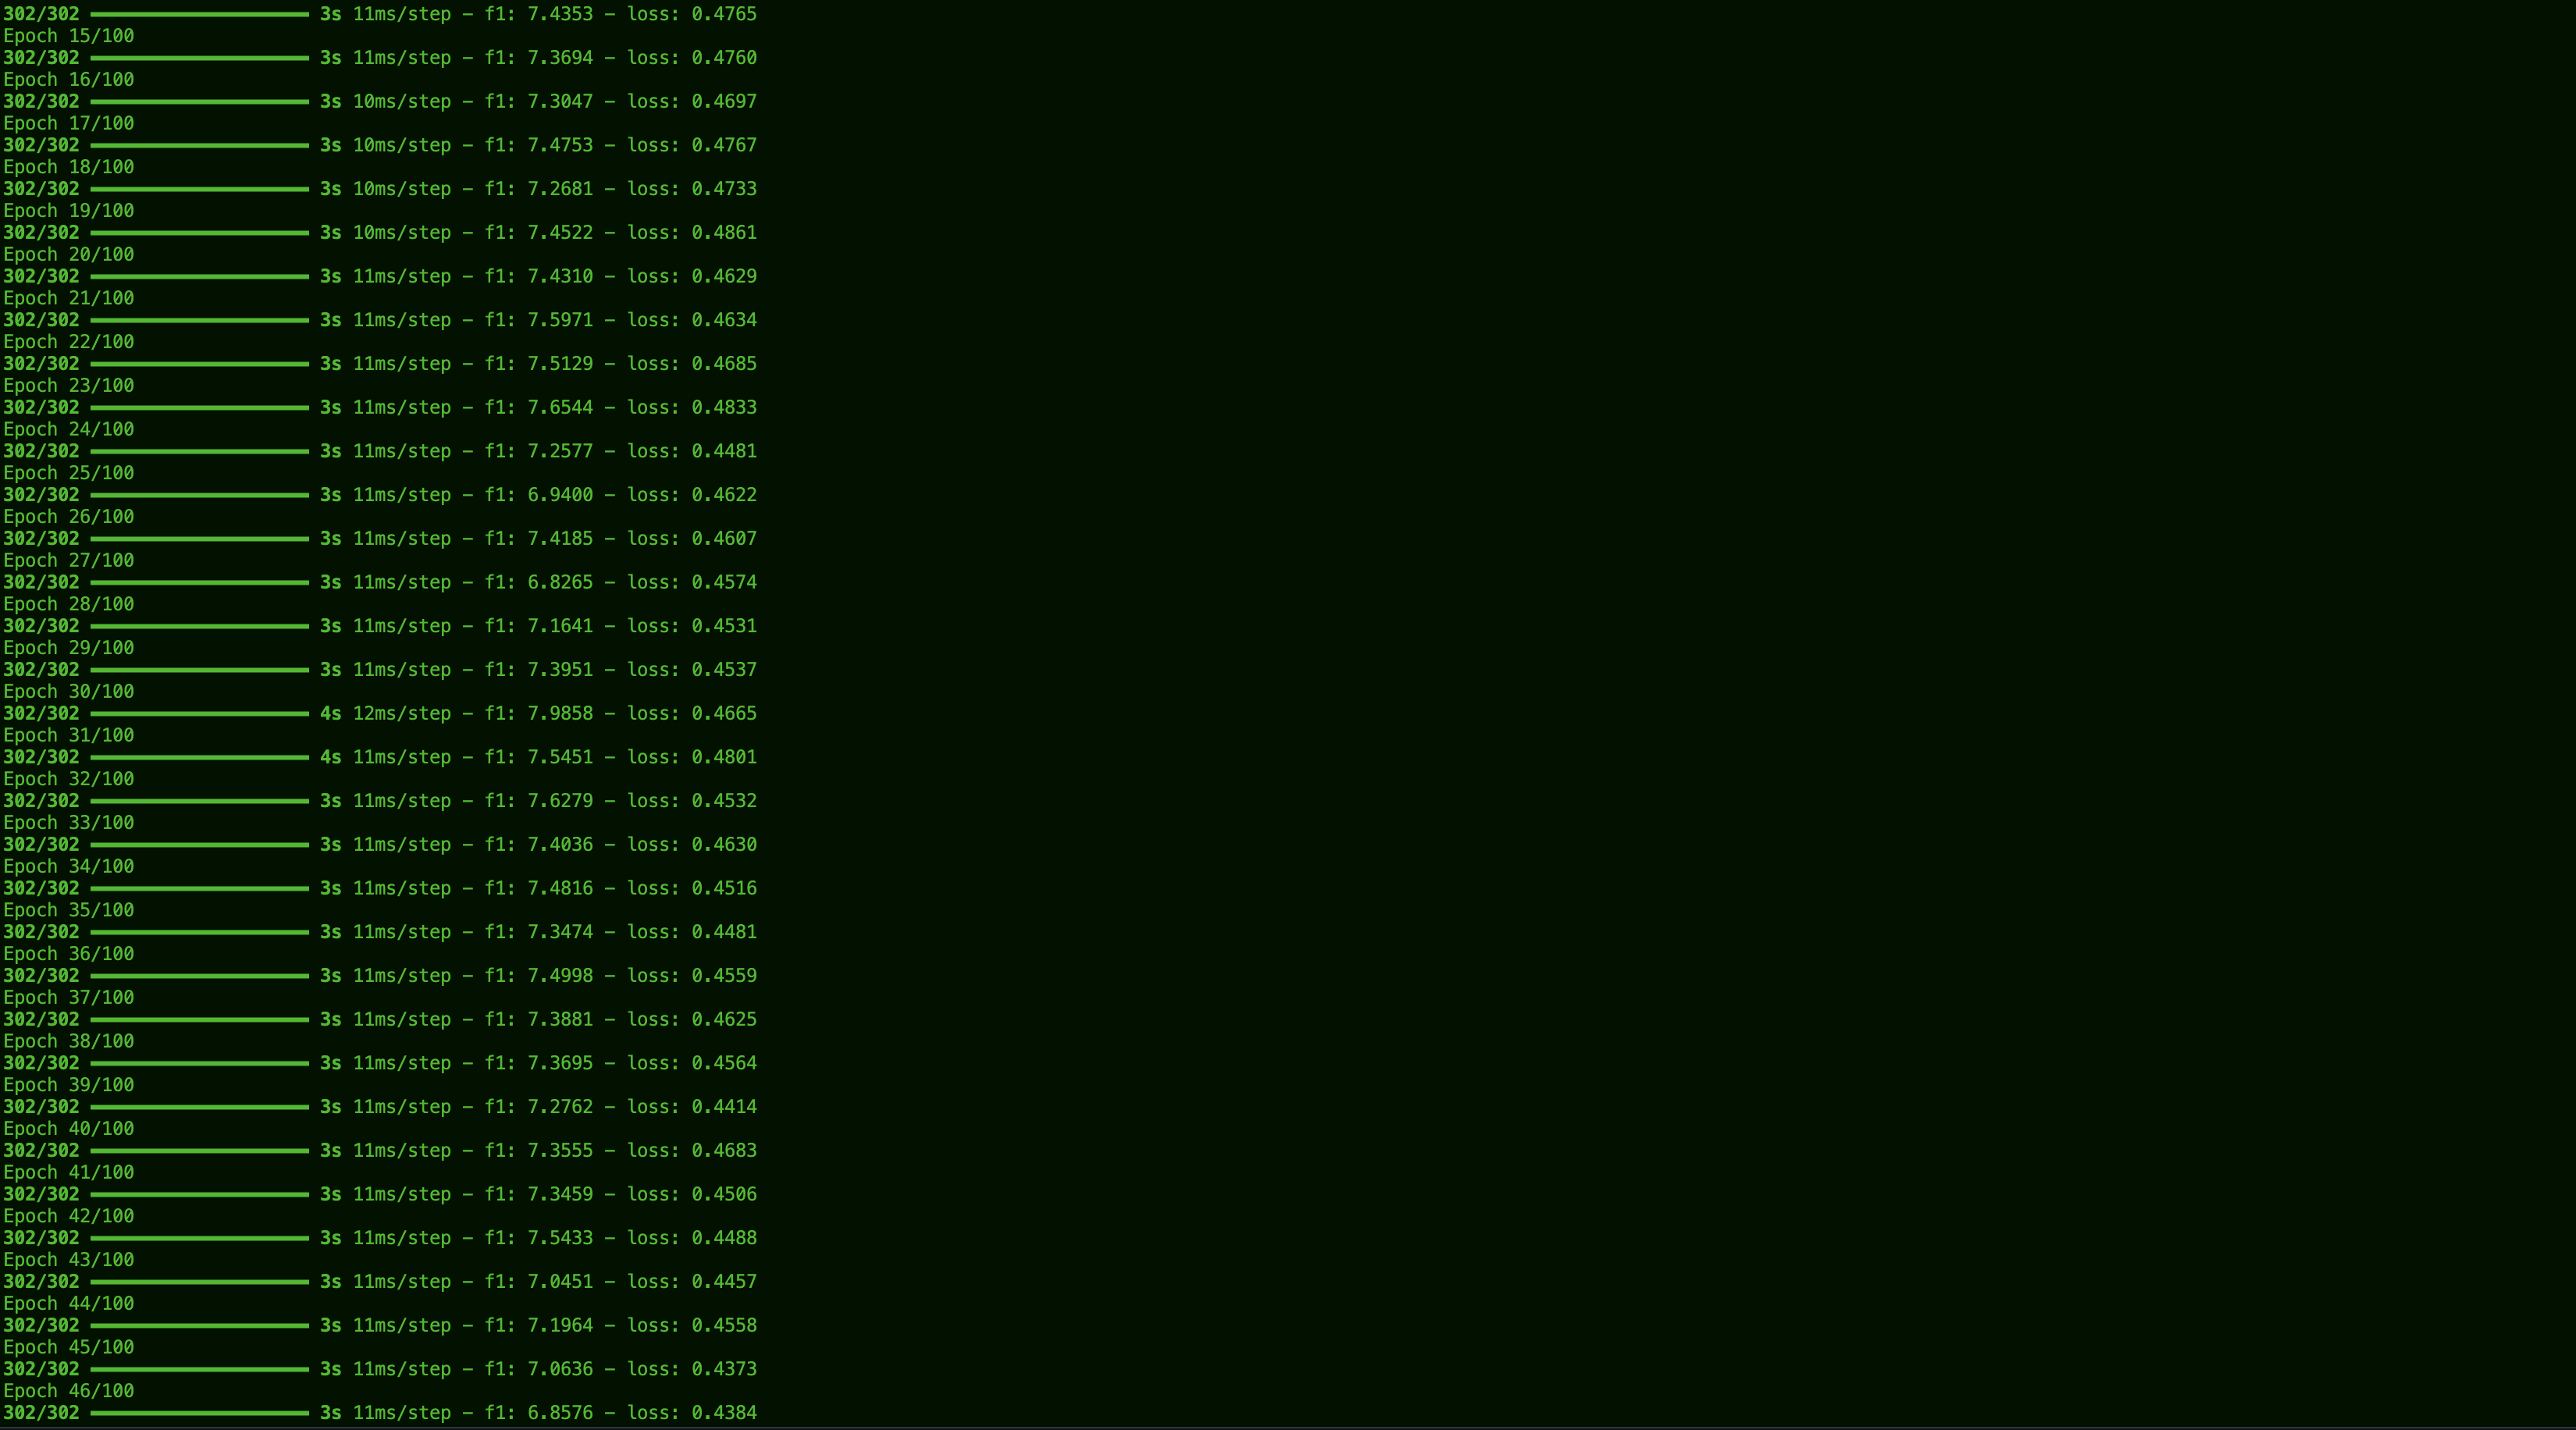
\includegraphics[width=1\linewidth]{makemodel2.png}
    \caption{The Epoch Steps Calculation}
    \label{fig:makemodel2}
\end{figure}
\begin{figure}
    \centering
    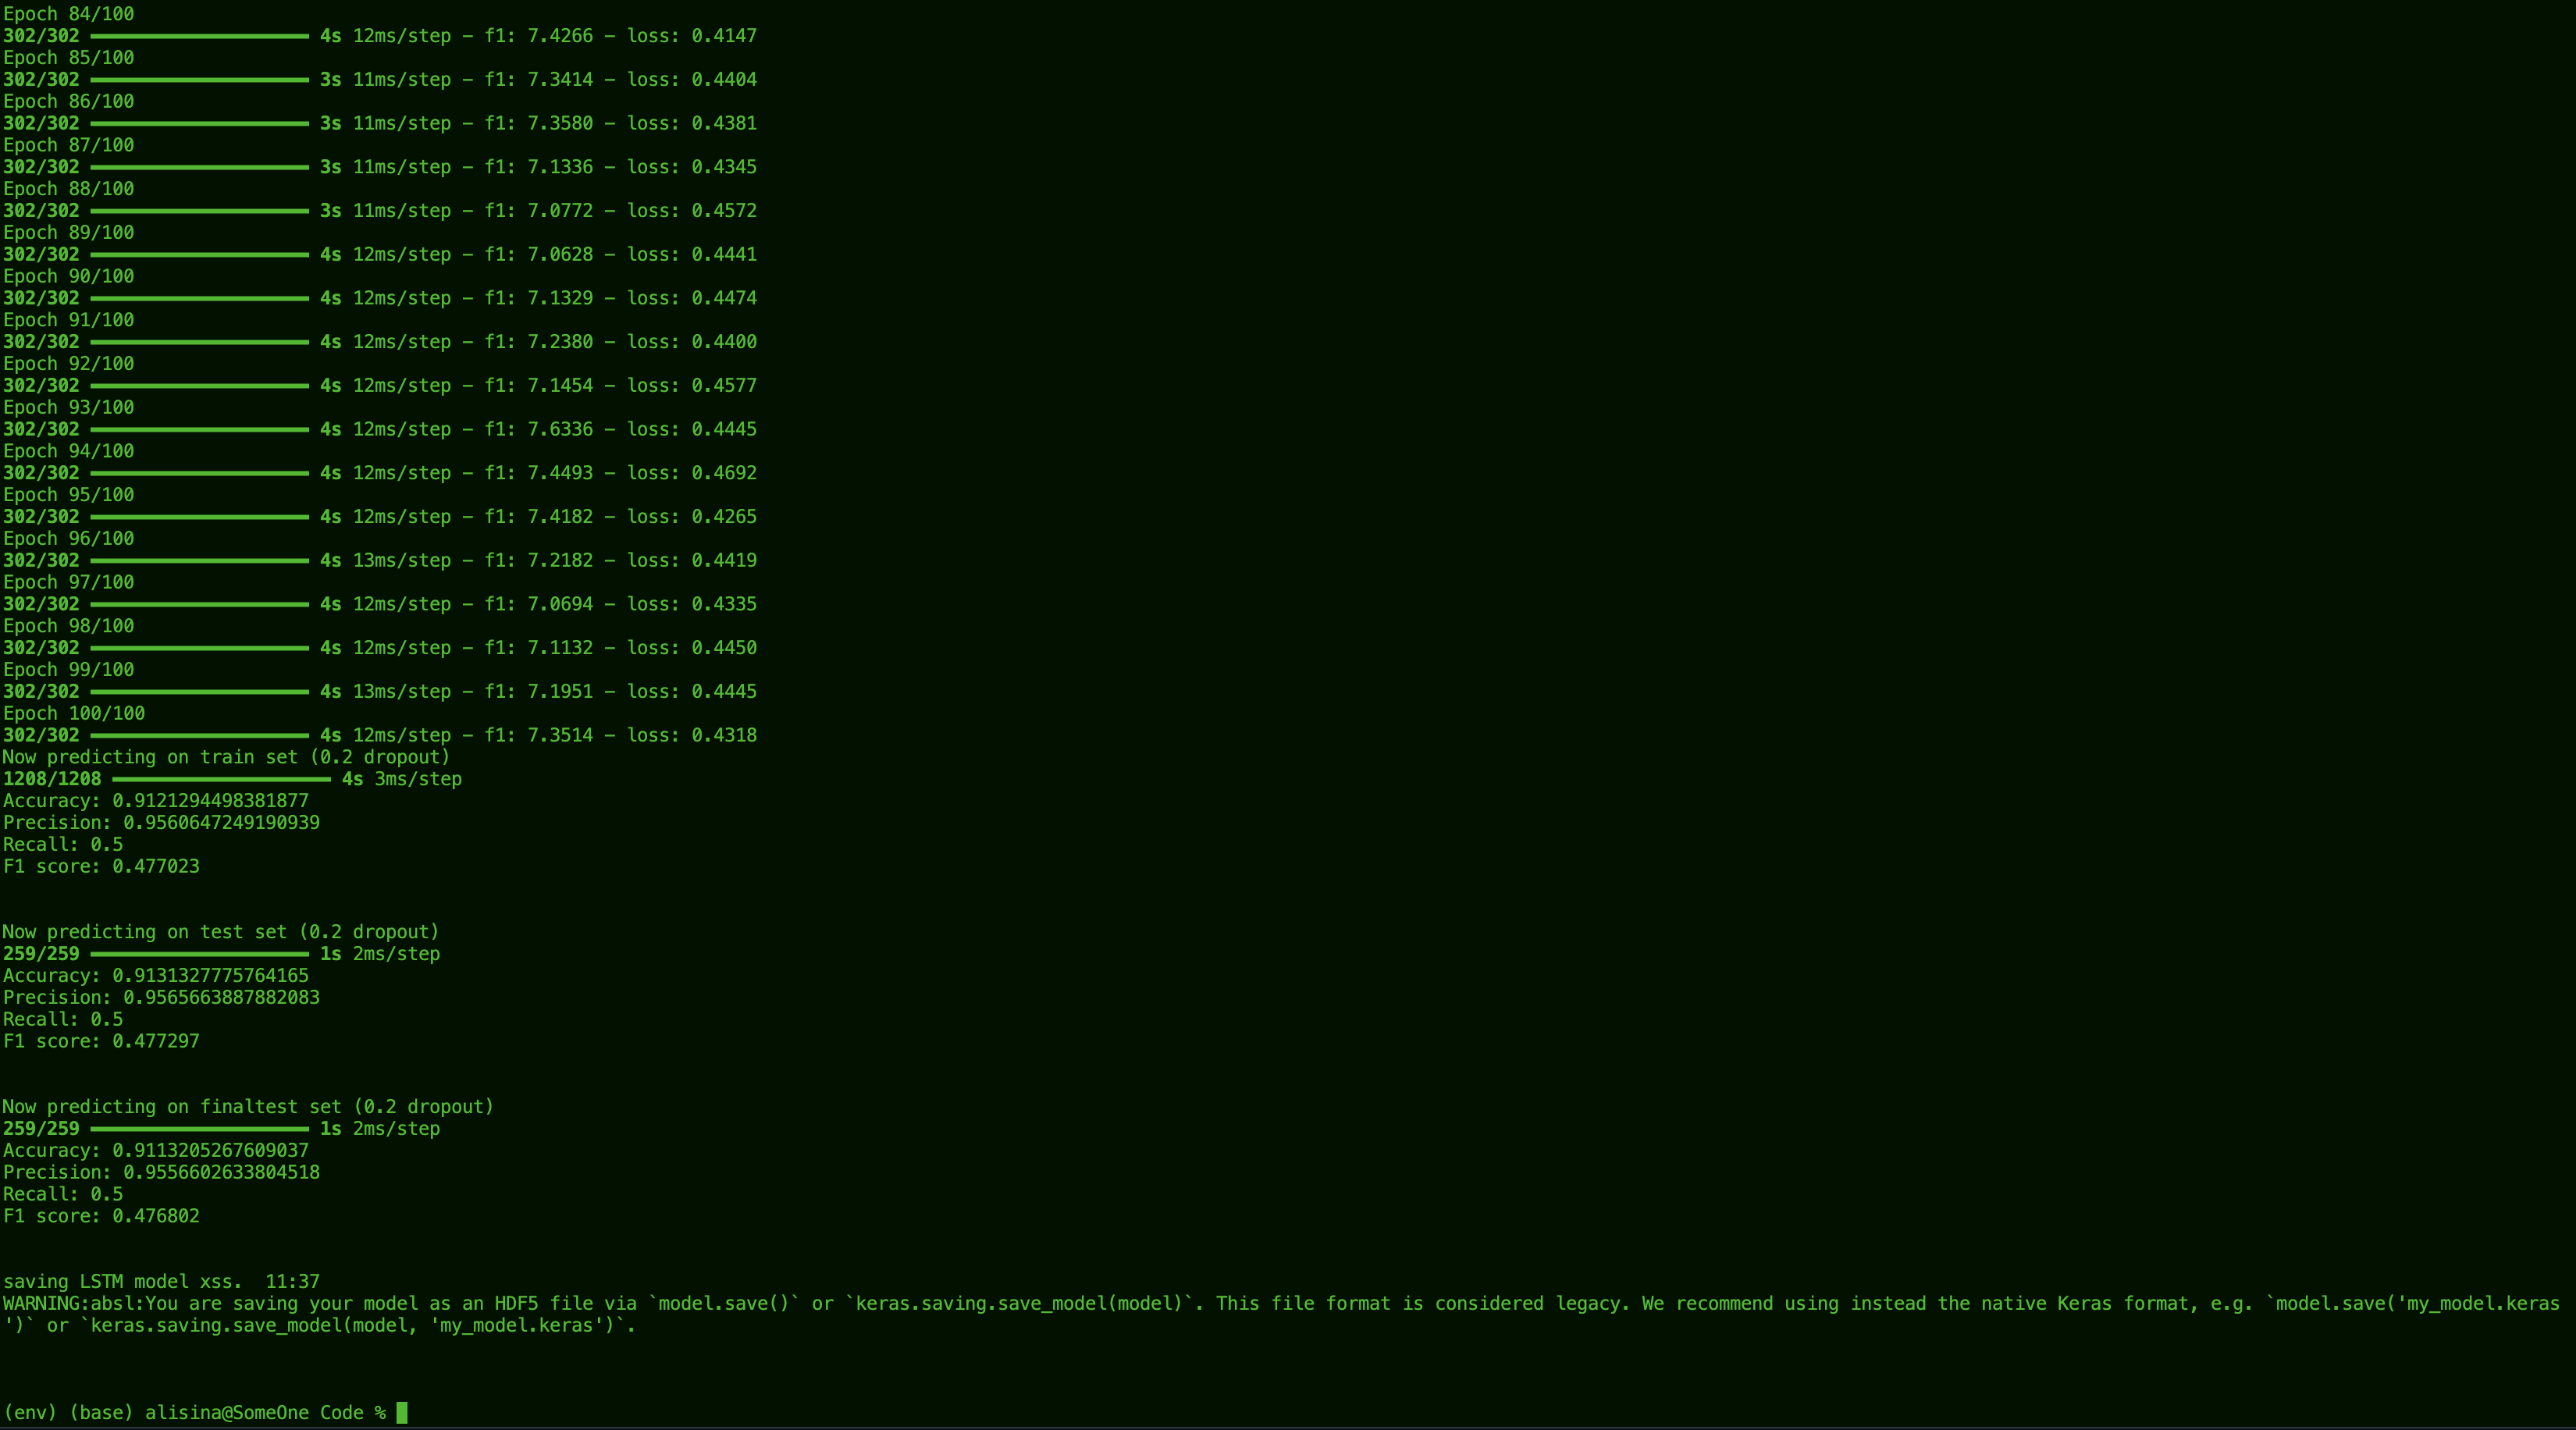
\includegraphics[width=1\linewidth]{makemodel3.png}
    \caption{Model Generation and Saving it}
    \label{fig:makemodel3}
\end{figure}
